\documentclass[twocolumn]{article}
\usepackage[english]{babel}
\usepackage[utf8]{inputenc}
\usepackage{amsmath,amssymb,physics,mathtools,blindtext,graphicx,float}
\usepackage[a4paper,total={7.5in,10in}]{geometry}
\usepackage[labelfont=bf]{caption}

\begin{document}
\begin{large}

\section*{TOV}
\subsection*{Introduction}
\begin{equation}
    \begin{split}
        &\frac{\text{d}P}{\text{d}r} = -\frac{G\left[P+\mathcal{E}(r)\right]\left[M(r)+4\pi r^3P/c^2\right]}{c^2r^2[1-2GM(r)/(c^2r)]} \\ 
        &\frac{\text{d}M}{\text{d}r} = 4\pi r^2\frac{\mathcal{E}(r)}{c^2}
    \end{split}
\end{equation}
An interpretation of these equations can be more readily seen by multiplying the first equation by $4\pi r^2\mathcal{E}\text{d}r/c^2 = \text{d}M$ and cancelling $\mathcal{E}$ on both sides:
\begin{equation}
    \label{28maj1039}
    \begin{split}
        4\pi r^2\text{d}P &= -\frac{GM\text{d}M}{r^2}\left(1+\frac{P}{\mathcal{E}(r)}\right)\left(1+\frac{4\pi r^3P}{Mc^2}\right) \\ 
        &\hspace{2cm}\times\left(1-\frac{2GM}{c^2r^2}\right)^{-1}
    \end{split}
\end{equation}
The term on the left hand side is the force exerted on a infinitesimal shell at radius $r$. The first factor on the right hand side is the newtonian gravitational force from the interior acting on this shell.

\subsection*{Equation of state}
\subsubsection*{\textit{Equation of state for a white dwarf:}}
In this model for a white dwarf, it is assumed that its matter content is composed of inert heavy nuclei (e.g. oxygen or carbon nuclei) in a sea of electrons. Due to the high density, the electrons are not bound to the nuclei and can move freely. Furthermore, it is assumed that the electrons form a zero temperature Fermi gas. From Fermi statistics, the number density of electrons is then given by
\begin{equation}
    \label{28maj0858}
    n = \frac{p_F^3}{3\pi^2\hbar^3}
\end{equation}
where $p_F$ is the Fermi momentum. The energy density is also given by 
\begin{equation}
    \mathcal{E}_e = 2\int\limits_0^{p_F}\sqrt{c^2p^2+m_e^2c^4}\frac{4\pi p^2}{(2\pi\hbar)^3}\text{d}p
\end{equation}
where $\sqrt{c^2p^2+m_e^2c^4}$ is the energy of an electron with momentum $p$ and mass $m_e$. By calculating this integral, one finds that 
\begin{equation}
    \label{28maj0910}
    \begin{split}
        &\mathcal{E}_e = \frac{(m_ec^2)^4}{8\pi^2(\hbar c)^3}\bigg[x_F\sqrt{1+x_F^2}\left(1+2x_F^2\right) \\ 
        &\hspace{2.75cm}-\ln\left(x_F+\sqrt{1+x_F^2}\right)\bigg] \\ 
    \end{split}
\end{equation}
where $x_F = cp_F/m_ec^2$. The total energy density is then the sum of the rest masses of the nuclei and $\mathcal{E}_e$,
\begin{equation}
    \label{28maj0852}
    \mathcal{E} = Ynm_pc^2 + \mathcal{E}_e,
\end{equation}
where $Y$ is the number of nuclei per electron ($Y=2$ for carbon and oxygen for example) and $m_p$ is the mass of the nuclei which is taken to be equal to the proton mass (the mass difference between the neutron and proton is neglected). Notice that equation \eqref{28maj0852} can be written exclusively in terms of $x_F$ by using equation \eqref{28maj0858} and $x_F=cp_F/m_ec^2$:
\begin{equation}
    \label{28maj1110}
    \begin{split}
        &\mathcal{E}=\frac{Y}{3\pi^2}\left(\frac{m_p}{m_e}\frac{(m_ec^2)^4}{(\hbar c)^3}\right)x_F^3 + \frac{(m_ec^2)^4}{8\pi^2(\hbar c)^3}F(x_F)
    \end{split}
\end{equation}
where $F$ is the function in the square brackets in equation \eqref{28maj0910}:
\begin{equation}
    \begin{split}
        F(x_F) &= x_F\sqrt{1+x_F^2}\left(1+2x_F^2\right) \\ 
        &\hspace{1cm}-\ln\left(x_F+\sqrt{1+x_F^2}\right).
    \end{split}
\end{equation}
From this we see that the rest mass term of the nuclei is substantially larger than the energy of the electrons since $m_p/m_e\sim 10^3$. 

Having found an expression for the energy density $\mathcal{E}$, we can find the pressure $P$ by utilizing the first law of thermodynamics and taking the derivative of the energy with respect to volume at zero temperature. By transforming this derivative to a derivative of the energy density with respect to the number density, we find that
\begin{equation}
    \label{28maj1025}
    \begin{split}
        P &= n\frac{\text{d}\mathcal{E}}{\text{d}n} - \mathcal{E} \\ 
        &= \frac{(m_ec^2)^4}{8\pi^2(\hbar c)^3}\bigg[\frac{2}{3}x_F^3\sqrt{1+x_F^2}-x_F\sqrt{1+x_F^2} \\ 
        &\hspace{2.90cm}+\ln\left(x_F+\sqrt{1+x_F^2}\right)\bigg] \\ 
        &= \frac{(m_ec^2)^4}{8\pi^2(\hbar c)^3}G(x_F)
    \end{split}
\end{equation}
where a function $G$ has been defined as the expression in the square brackets. Notice that the energy density and pressure differ by order of magnitude $\mathcal{E}/P\sim m_p/m_e\sim 10^3$. Now we know both $\mathcal{E}$ and $P$ as functions of $x_F$ (which in turn is a function of the number density $n$) but we don't have an explicit expression for the function $\mathcal{E}(P)$. Given a pressure $P=P_0$ we can however use a root finding algorithm to find the $x_F$ such that $P(x_F) - P_0 = 0$. Having found this value $x_F$, we can plug it into the equation for the energy density to find $\mathcal{E}(P_0)$. 

\subsubsection*{\textit{Equation of state for a neutron star}}
The model which will be used for a neutron star is somewhat simpler than the one for the white dwarf and the equation for the energy density and pressure will be the similar as the ones above. It will be assumed that the equation of state is that of a degenerate gas of non-interacting neutrons at zero temperature. Hence, the energy density will be the same as the one for the electrons in equation \eqref{28maj0910} but with the neutron mass $m_n$ instead of the electron mass:
\begin{equation}
    \mathcal{E}_n = \frac{(m_nc^2)^4}{8\pi^2(\hbar c)^3}F(y_F)
\end{equation}
where $y_F = cp_F/m_nc^2$. The pressure is found in the same way as above and is given by equation \eqref{28maj1025} with the electron mass exchanged for the neutron mass:
\begin{equation}
    P = \frac{(m_nc^2)^4}{8\pi^2(\hbar c)^3}G(y_F).
\end{equation}
In this model of the neutron star the energy density and pressure are of the same order of magnitude which implies that the relativistic corrections in the TOV-equations \eqref{28maj1039} are important.


%\begin{equation}
%    \label{24maj2054}
%    \begin{split}
%        &\mathcal{E}(n) = \frac{(mc^2)^4}{8\pi^2(\hbar c)^3}\bigg[x_F\sqrt{1+x_F^2}\left(1+2x_F^2\right) \\ 
%        &\hspace{2.75cm}-\ln\left(x_F+\sqrt{1+x_F^2}\right)\bigg] \\ 
%        &P(n) = \frac{(mc^2)^4}{8\pi^2(\hbar c)^3}\bigg[\frac{2}{3}x_F^3\sqrt{1+x_F^2}-x_F\sqrt{1+x_F^2} \\ 
%        &\hspace{2.90cm}+\ln\left(x_F+\sqrt{1+x_F^2}\right)\bigg]
%    \end{split}
%\end{equation}
%where $x_F(n)=\hbar c(3\pi n)^{1/3}/(mc^2)$.

\subsection*{Numerical set-up}
\subsubsection*{\textit{Rescaling the TOV-equations}}
The TOV-equations can be made more suitible for numerical calculations by rescaling the variables. Making the substitutions  
\begin{equation*}
    \begin{split}
        &r = R_0x \quad P=P_0p \\ 
        &\mathcal{E} = \mathcal{E}_0\varepsilon \quad M = M_0m
    \end{split}
\end{equation*}
the equation for the pressure can be written
\begin{equation}
    \begin{split}
        &\left(\frac{P_0}{R_0}\right)\frac{\text{d}p}{\text{d}x} = -\left(\frac{G\mathcal{E}_0M_0}{c^2R_0^2}\right) \\ 
        &\hspace{1cm}\times \frac{\left[(P_0/\mathcal{E}_0)p+\varepsilon\right]\left[m+4\pi R_0^3x^3P_0p/(c^2M_0)\right]}{x^2\left[1-2GM_0m/(c^2R_0x)\right]}.
    \end{split}
\end{equation}
Dividing by $P_0/R_0$ on both sides yields
\begin{equation}
    \label{28maj1116}
    \begin{split}
        &\frac{\text{d}p}{\text{d}x} = -\left(\frac{GM_0}{c^2R_0}\right)\left(\frac{\mathcal{E}_0}{P_0}\right) \\ 
        &\hspace{1cm}\times \frac{\left[(P_0/\mathcal{E}_0)p+\varepsilon\right]\left[m+4\pi R_0^3x^3P_0p/(M_0c^2)\right]}{x^2\left[1-2GM_0m/(c^2R_0x)\right]}.
    \end{split}
\end{equation}
Similarily, the equation for the mass becomes
\begin{equation}
    \label{28maj1130}
    \frac{\text{d}m}{\text{d}x} = \left(\frac{4\pi R_0^3\mathcal{E}_0}{M_0c^2}\right)x^2\varepsilon.
\end{equation}
Since the relation between energy density and pressure differs between a white dwarf and a neutron star, ($\mathcal{E}/P\sim 10^3$ for a white dwarf but $\mathcal{E}/P\sim 1$ for a neutron star), it is best to choose different scalings for the different type of stars.

\textit{White dwarf scaling:} Here we set the energy density scale as the term in the parenthesis in equation \eqref{28maj1110} and the pressure as $P_0 = (m_e/m_p)\mathcal{E}_0$:
\begin{equation}
\begin{split}
    &\mathcal{E}_0 = \frac{m_p}{m_e}\frac{(m_ec^2)^4}{(\hbar c)^3} = 16.294\text{ eV/fm}^3 , \\ 
    &P_0 = \frac{(m_ec^2)^4}{(\hbar c)^3} = 8.874\text{ meV/fm}^3.
    \end{split}
\end{equation}
The length scale and mass scale are then chosen such that the multiplication of the first two factors in equation \eqref{28maj1116} for the pressure becomes
\begin{equation}
    \label{28maj1119}
    \left(\frac{GM_0}{c^2R_0}\right)\left(\frac{\mathcal{E}_0}{P_0}\right) = 1.
\end{equation}
Let's set $M_0$ to be the mass of the sun, 
\begin{equation}
    M_0 = M_\odot = 1.99\cdot 10^{30} \text{ kg}
\end{equation}
which is comparable to the mass of a white dwarf. Equation \eqref{28maj1119} then fixes the length scale:
\begin{equation}
    R_0 = 2711 \text{ km}.
\end{equation}
Inserting these constants into the scaled TOV-equations \eqref{28maj1116} $-$ \eqref{28maj1130} yields:
\begin{equation}
    \begin{split}
        &\frac{\text{d}p}{\text{d}x} = -\frac{(\varepsilon + (m_e/m_p)p)(m+\mu x^3p)}{x(x-2(m_e/m_p)m)} \\ 
        &\frac{\text{d}m}{\text{d}x} = \nu x^2\varepsilon
    \end{split}
\end{equation}
where 
\begin{equation}
    \mu = 1.992\cdot 10^{-3},\quad \nu = 3.658.
\end{equation}
The variables $\mu$ and $m_e/m_p$ are associated with the relativistic correction to the Newtonian hydrostatic equations and when they are set equal to zero, the TOV-equations reduce to those equations. The variable $\nu$ is simply a result of the scaling and is also present in the Newtonian case.

\textit{Neutron star scaling:}
A natural choice for $\mathcal{E}_0$ and $P_0$ for the neutron star is
\begin{equation}
    \mathcal{E}_0 = P_0 = \frac{(mc^2)^4}{8\pi^2(\hbar c)^3} = 1.285 \text{ GeV/fm}^3.
\end{equation}
The scaled TOV-equations \eqref{28maj1116} $-$ \eqref{28maj1130} then simplify substantially if the numerical constants are chosen such that
\begin{equation}
    \label{26maj1005}
    1 = \frac{GM_0}{c^2R_0} = \frac{4\pi R_0^3P_0}{M_0c^2}.
\end{equation}
This fixes $M_0$ and $R_0$:
\begin{equation}
    \begin{split}
    &M_0 = 4.63 \text{ M}_\odot \\ 
    &R_0 = 6.84 \text{ km},
    %&M_0 = \sqrt{\frac{c^8}{4\pi\mathcal{E}_0G^3}} = 4.63 \text{ M}_\odot \\ 
    %&R_0 = \frac{GM_0}{c^2} = 6.84 \text{ km},
    \end{split}
\end{equation}
and the TOV-equations become
\begin{equation}
    \label{24maj1640}
    \begin{split}
        &\frac{\text{d}p}{\text{d}x} = -\frac{(p+\varepsilon)(m+x^3p)}{x(x-2m)} \\  %= f(p,\epsilon,m;x) \\ 
        &\frac{\text{d}m}{\text{d}x} = x^2\varepsilon. %= g(\epsilon;x)
    \end{split}
\end{equation}
It is apparent from these equations that relativistic corrections are important for a neutron star. 

\subsubsection*{\textit{Initial conditions}}
To solve these equations, initial conditions for both $p$ and $m$ are needed. From a physical consideration it is obvious to set $m(0)=0$. The initial value for the pressure can be either $p(0) = p_0$ or $p(x_0) = 0$ where $p_0$ is the pressure at the center of the star and $x_0$ is its radius. When $\varepsilon$ depends on the pressure $p$, it becomes easier to make use of the former condition since $m$ is integrated from the center. The equation for $p$ is however singular for $x=0$, so the equations have to be integrated from some value $\Delta x$ close to zero. Since the first two derivatives of $m$ are zero at $x=0$, the error of setting $m(\Delta x) = 0$ is of the order $(\Delta x)^3$.

Another thing which is needed is the equation of state $\epsilon(p)$ which, for the case of an ideal Fermi gas at zero temperature, can not be found directly but in terms of the number density $n$:
\begin{equation}
    \label{24maj1641}
    \begin{split}
        &\varepsilon(n) = x_F\sqrt{1+x_F^2}\left(1+2x_F^2\right)-\ln\left(x_F+\sqrt{1+x_F^2}\right) \\ 
        &p(n) = \frac{2}{3}x_F^3\sqrt{1+x_F^2}-x_F\sqrt{1+x_F^2} \\ 
        &\hspace{3.75cm}+\ln\left(x_F+\sqrt{1+x_F^2}\right)
    \end{split}
\end{equation}
with $x_F(n)=\hbar c(3\pi n)^{1/3}/(mc^2)$. Hence, for a given $p=p_0$ we need a root finding algorithm to find $n=n_0$ such that $p(n_0) = p_0$. Once $n_0$ has been found, we can plug that into $\varepsilon$ to find $\varepsilon(n_0)=\varepsilon(p_0)$. 

Having set up the equations which are to be integrated \eqref{24maj1640} and the equation of state \eqref{24maj1641}, the following steps were taken to solve the TOV-equations: 
\begin{itemize}
    \item[1.] Set the initial conditions by specifying $p(\Delta x) = p_c = p_{j=0}$ and set $m(\Delta x) = 0 = m_{j=0}$.
    \item[2.] Find the energy density by using the bisection method on $p(n) = p_j$ and plugging $n$ into the equation for the energy density to get $\epsilon(n)=\varepsilon_j$. 
    \item[3.] Use Heun's integration method on \eqref{24maj1640} to obtain $p_{j+1}$ and $m_{j+1}$. 
    \item[4.] Repeat from 2. until the pressure is zero, $p_{j+1}=0$.
\end{itemize}
The step size used was $h=10^{-4}$ and the tolerance for the bisection method was $\Delta = 10^{-8}$. 

\subsection*{Results}
\begin{center}
    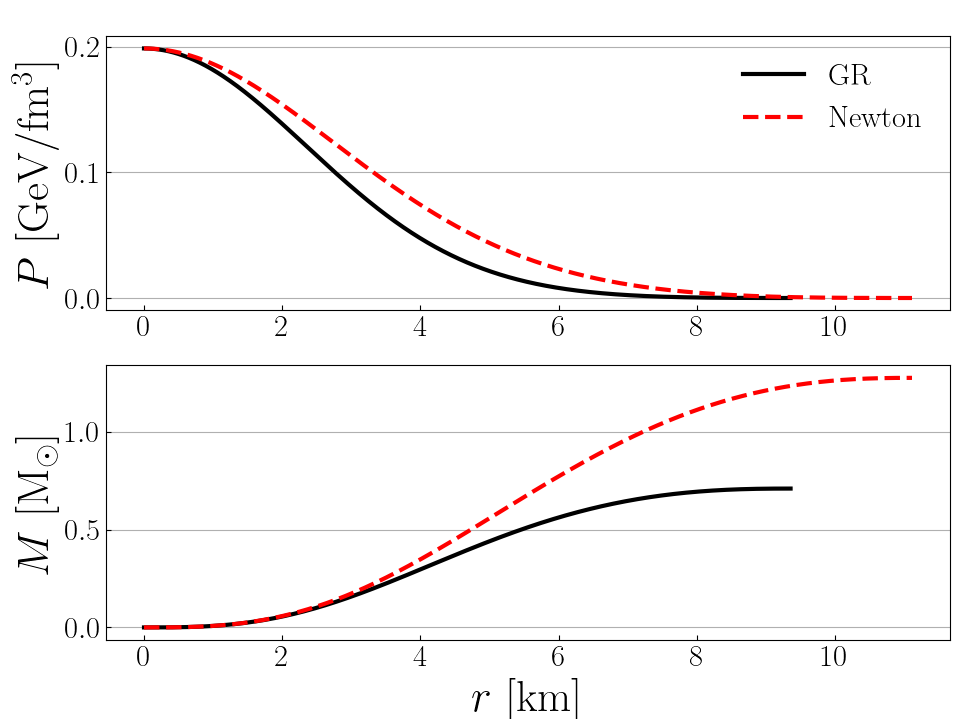
\includegraphics[scale=0.35]{Newt.png}
\end{center}
\begin{center}
    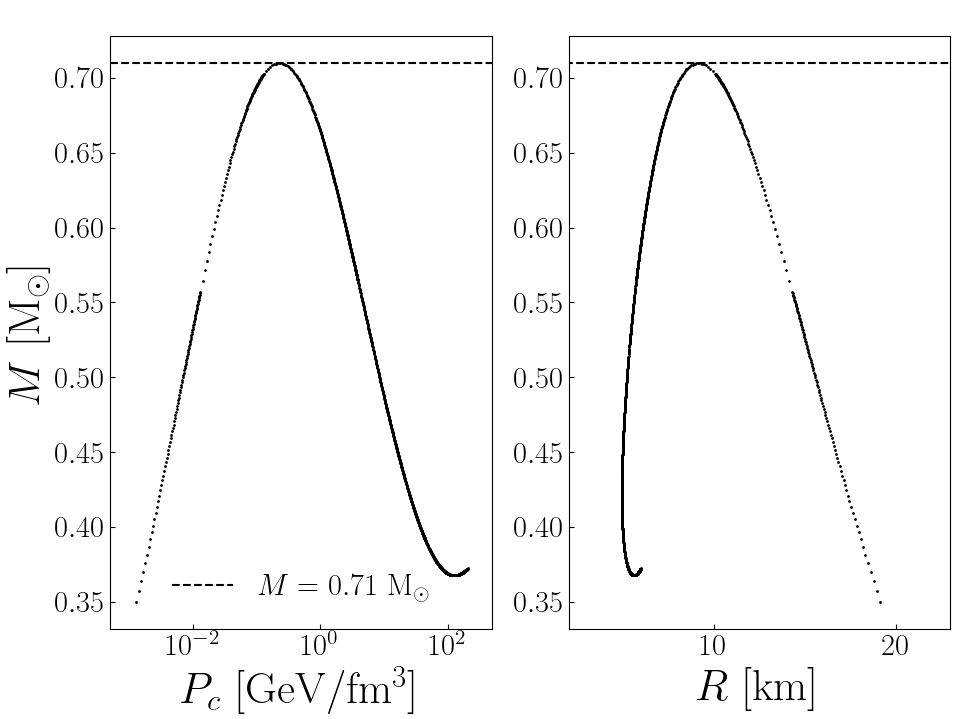
\includegraphics[scale=0.35]{TOV_limit.png}
\end{center}



\subsection*{Notes}
\begin{itemize}
    \item Compare with Newton  (x)
    \item Also do white dwarfs (x)
    \item Remove equation numberings which are not needed
\end{itemize}




\end{large}
\end{document}
